% <!-- coding: utf-8 -->
\renewcommand{\monlhead}{Données ornitho faune-bretagne}
\section*{Présentation}
Les données sont extraites de faune-bretagne sur la zone géographique -1.775795/48.105037 -1.711859/48.060601

Cette extraction est faite en format csv. Les données sont ensuite traitées en R

Un rapprochement est effectué avec le référenciel taxonomique TAXREF.
Les espèces spécifiques à biolovision ne sont pas prises en compte.

Les familles sont différentes pour certaines espèces, en version 9.0 de TAXREF :
\begin{itemize}
\item Roitelet à triple bandeau   Sylviidae   Regulidae
\item Rougegorge familier    Turdidae Saxicolidae
\end{itemize}

Des statistiques sont produites pour les données :
\begin{itemize}
\item sur la zone d'extraction
\item sur la période 1er décembre - 20 janvier
\item sur la période 1er décembre 2016 - 20 janvier 2017
\end{itemize}
\vfill \null
\section*{Statistiques zone d'extraction}
\subsection*{par famille}
\mongraphique{images/faune_stat_champ_FAMILY_NAME_prec.pdf}
\subsection*{par année}
\mongraphique{images/faune_stat_champ_annee_prec.pdf}
\subsection*{par mois}
\mongraphique{images/faune_stat_champ_mois_prec.pdf}
\subsection*{par type de localisation}
\mongraphique{images/faune_stat_champ_PRECISION_prec.pdf}

\section*{Statistiques 1er décembre - 20 janvier}
\subsection*{par famille}
\mongraphique{images/faune_stat_champ_FAMILY_NAME_hiver.pdf}
\subsection*{par année}
\mongraphique{images/faune_stat_champ_annee_hiver.pdf}
\subsection*{par mois}
\mongraphique{images/faune_stat_champ_mois_hiver.pdf}
\subsection*{par type de localisation}
\mongraphique{images/faune_stat_champ_PRECISION_hiver.pdf}

\section*{Statistiques 1er décembre - 20 janvier - atlas}
\subsection*{par famille}
\mongraphique{images/faune_stat_champ_FAMILY_NAME_hiver_atlas.pdf}
\subsection*{par année}
\mongraphique{images/faune_stat_champ_annee_hiver_atlas.pdf}
\subsection*{par mois}
\mongraphique{images/faune_stat_champ_mois_hiver_atlas.pdf}
\subsection*{par type de localisation}
\mongraphique{images/faune_stat_champ_PRECISION_hiver_atlas.pdf}

\section*{Statistiques 1er décembre 2016 - 20 janvier 2017}
\subsection*{par famille}
\mongraphique{images/faune_stat_champ_FAMILY_NAME.pdf}
\subsection*{par famille taxref}
\mongraphique{images/faune_stat_champ_FAMILLE.pdf}
\subsection*{par ordre taxref}
\mongraphique{images/faune_stat_champ_ORDRE.pdf}
\subsection*{par espèce}
\mongraphique{images/faune_stat_champ_NAME_SPECIES.pdf}
\subsection*{par date}
\mongraphique{images/faune_stat_champ_d.pdf}
\subsection*{par observateur}
\mongraphique{images/faune_stat_champ_observateur.pdf}
\subsection*{par lieudit}
\mongraphique{images/faune_stat_champ_PLACE.pdf}
\subsection*{par type de localisation}
\mongraphique{images/faune_stat_champ_PRECISION.pdf}
\clearpage
\section*{Carte}
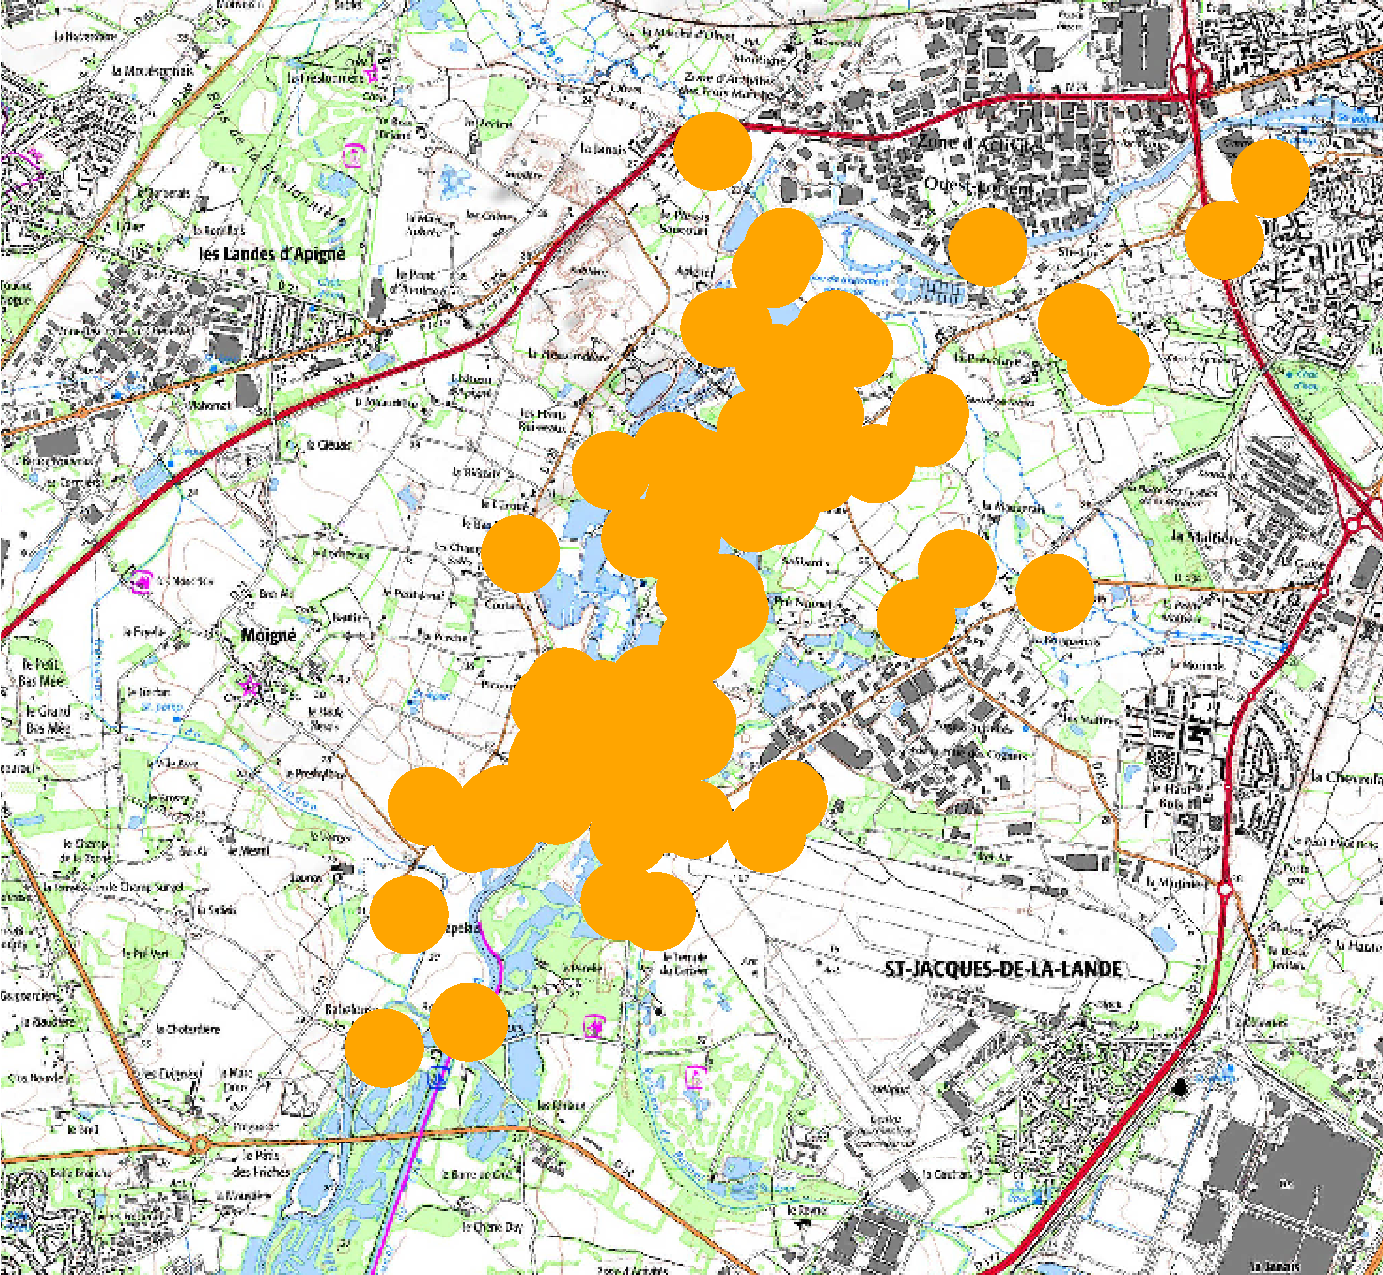
\includegraphics[width=\textwidth]{images/faune_carte.pdf}